\section{Dokumentacija naudotojui}

Šis skyrius skirtas skaitmeninės logikos inžinieriams, \glsdisp{verification}{verifikacijos} specialistams bei sistemų administratoriams, dirbantiems su kuriamu \glsdisp{microprocessor}{mikrovaldiklio} \glsdisp{verification}{verifikavimo} \glsdisp{framework}{karkasu}. Čia pateikiama visa reikalinga informacija pradedant nuo aukšto lygio sistemos galimybių apžvalgos, baigiant detaliomis instrukcijomis, kaip įdiegti, konfigūruoti ir naudoti sistemą kasdieniame darbe.

\subsection{Apibendrintas sistemos galimybių aprašymas}

Kuriamas \glsdisp{verification}{verifikavimo} \glsdisp{framework}{karkasas} yra universalus įrankių rinkinys, leidžiantis automatizuotai testuoti \gls{risc} architektūros mikrovaldiklį. Naudotojui nereikia gilintis į sudėtingą \gls{eda} įrankių konfigūraciją ar priklausomybių valdymą operacinėje sistemoje -- visa tai atliekama automatizuotai. Pagrindinės sistemos galimybės, kurias gali išnaudoti naudotojas:
\begin{itemize}
	\item \textbf{Universalus testų paleidimas:} Galimybė leisti \textit{Python} (\textit{PyUVM}) testus nepriklausomai nuo operacinės sistemos, naudojant izoliuotus \textit{Docker} arba \textit{Podman} \glsdisp{container}{konteinerius}.
	\item \textbf{Skirtingų imituoklių palaikymas:} Laisvas pasirinkimas tarp atviros prieigos nemokamos \textit{Verilator} \glsdisp{simulator}{imituoklės} (tinkamos greitam testavimui vietiniame kompiuteryje) ir komercinės \textit{Cadence Xcelium} (skirtos sudėtingoms ir tikslioms imitacijoms serveryje).
	\item \textbf{Aparatinės ir programinės įrangos integracija:} Karkasas automatiškai sukompiliuoja C kalba aprašytą mikrovaldiklio programinę įrangą ir įkelia ją į \gls{dut} atmintį prieš pradedant imitaciją.
	\item \textbf{Vaizdinė signalų ir metrikų analizė:} Integruotas automatinis signalų (\glsdisp{waveform}{laikinių diagramų}) išsaugojimas ir peržiūra naudojant \textit{GTKWave} arba \textit{SimVision} įrankius, bei \glsdisp{functional-coverage}{funkcinio padengiamumo} ataskaitų generavimas.
	\item \textbf{Patogi darbo aplinka:} Specialiai paruoštas \textit{Tmux} terminalo scenarijus, kuris padalina ekraną į patogias sekcijas kodo rašymui, komandų vykdymui ir transakcijų stebėjimui realiu laiku.
\end{itemize}

\subsection{Diegimo vadovas}

Prieš pradedant darbą su \glsdisp{verification}{verifikavimo} aplinka, būtina ją paruošti pagrindinėje kompiuterio operacinėje sistemoje. Šis vadovas skirtas standartiniam naudotojui, dirbančiam su atviros prieigos įrankiais (pvz., per \gls{wsl} ar \textit{Linux}). 

\textbf{Sistemos reikalavimai:}
\begin{itemize}
	\item Operacinė sistema: \textit{Linux} (rekomenduojama \textit{Ubuntu/Debian}), \textit{macOS} arba \textit{Windows} (tik per \gls{wsl}).
	\item Įdiegta programinė įranga: \textit{Git}, \textit{GNU Make} (v4.3+), \textit{Docker} (v24+). Naudotojas turi turėti teises vykdyti \textit{Docker} komandas (būti \texttt{docker} naudotojų grupėje).
\end{itemize}

\textbf{1 žingsnis. Projekto atsisiuntimas ir pataisų pritaikymas} \\
Klonuokite pagrindinę mikrovaldiklio kodo saugyklą iš \textit{\href{https://github.com/ktu-proto-lab/mlab_mcu_pyuvm}{GitHub}} ir pereikite į \glsdisp{verification}{verifikacijos} karkaso katalogą. Kadangi karkasas veikia kaip \glsdisp{plugin}{įskiepis}, pritaikykite suderinamumo pataisas šakniniam projektui:
\begin{lstlisting}[basicstyle=\ttfamily\footnotesize, language=bash]
$ git clone --recurse-submodules <repo_url> mlab_mcu
$ cd mlab_mcu/uvm
$ git checkout main
$ make patch apply
\end{lstlisting}

\begin{figure}[H]
	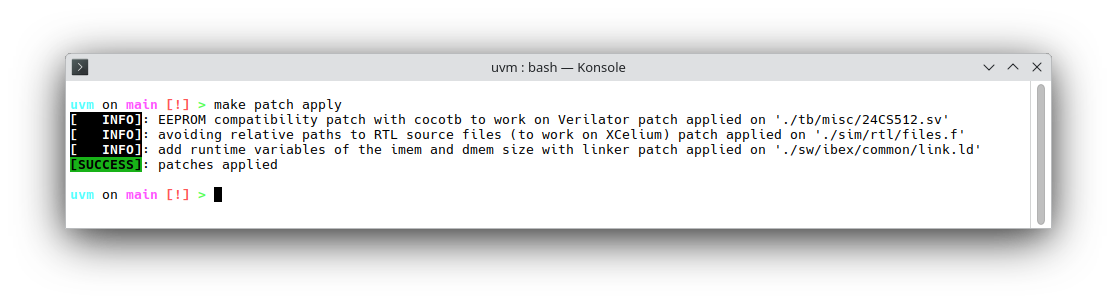
\includegraphics[width=\linewidth]{images/doc_make_patch_apply.png}
	\caption{Sėkmingas suderinamumo pataisų pritaikymas šakniniam projektui}
	\label{fig:doc_make_patch_apply}
\end{figure}

\textbf{2 žingsnis. Konteinerio atvaizdo surinkimas} \\
Surinkite izoliuotą \textit{Verilator} \glsdisp{simulator}{imituoklės} aplinką. Šis procesas automatiškai atsisiųs reikiamus \textit{Ubuntu} paketus, C kompiliatorius ir \textit{Verilator} įrankį. Tai gali užtrukti keletą minučių:
\begin{lstlisting}[basicstyle=\ttfamily\footnotesize, language=bash]
$ make image verilator
\end{lstlisting}

\begin{figure}[H]
	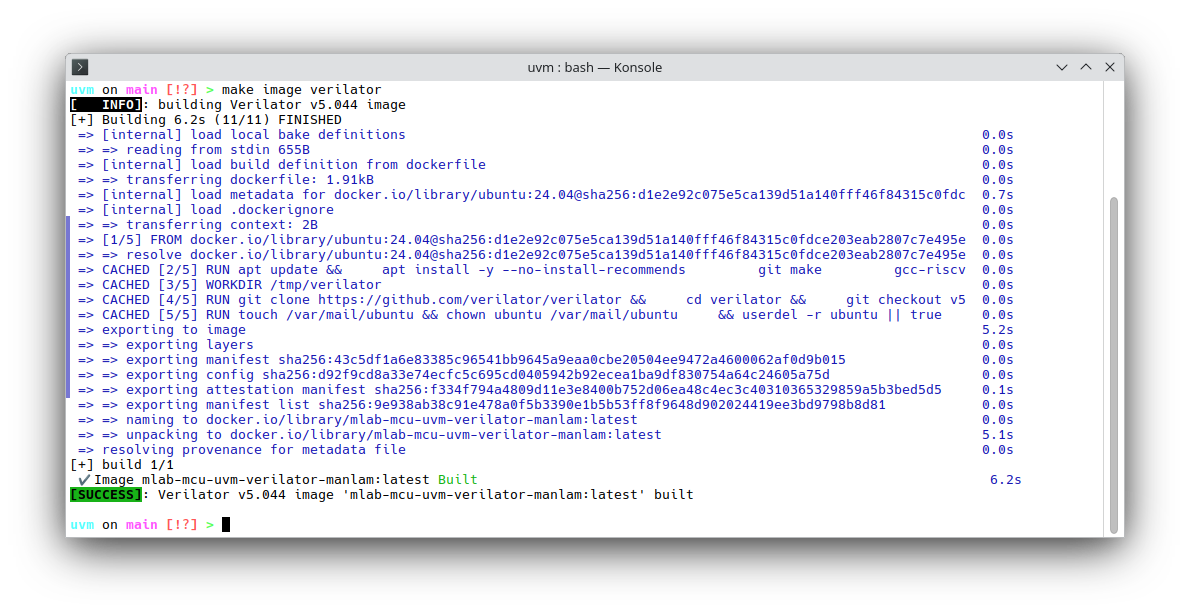
\includegraphics[width=\linewidth]{images/doc_make_image_verilator.png}
	\caption{Sėkmingas \textit{Verilator} atvaizdo surinkimas naudojant \textit{Make} skriptą}
	\label{fig:doc_make_image_verilator}
\end{figure}

\textbf{3 žingsnis. Python virtualios aplinkos paruošimas} \\
Sukonfigūruokite \textit{Python} testavimo priklausomybes (\textit{Cocotb}, \textit{PyUVM}). Karkasas automatiškai sukurs \texttt{.venv} katalogą:
\begin{lstlisting}[basicstyle=\ttfamily\footnotesize, language=bash]
$ make venv verilator
\end{lstlisting}

\begin{figure}[H]
	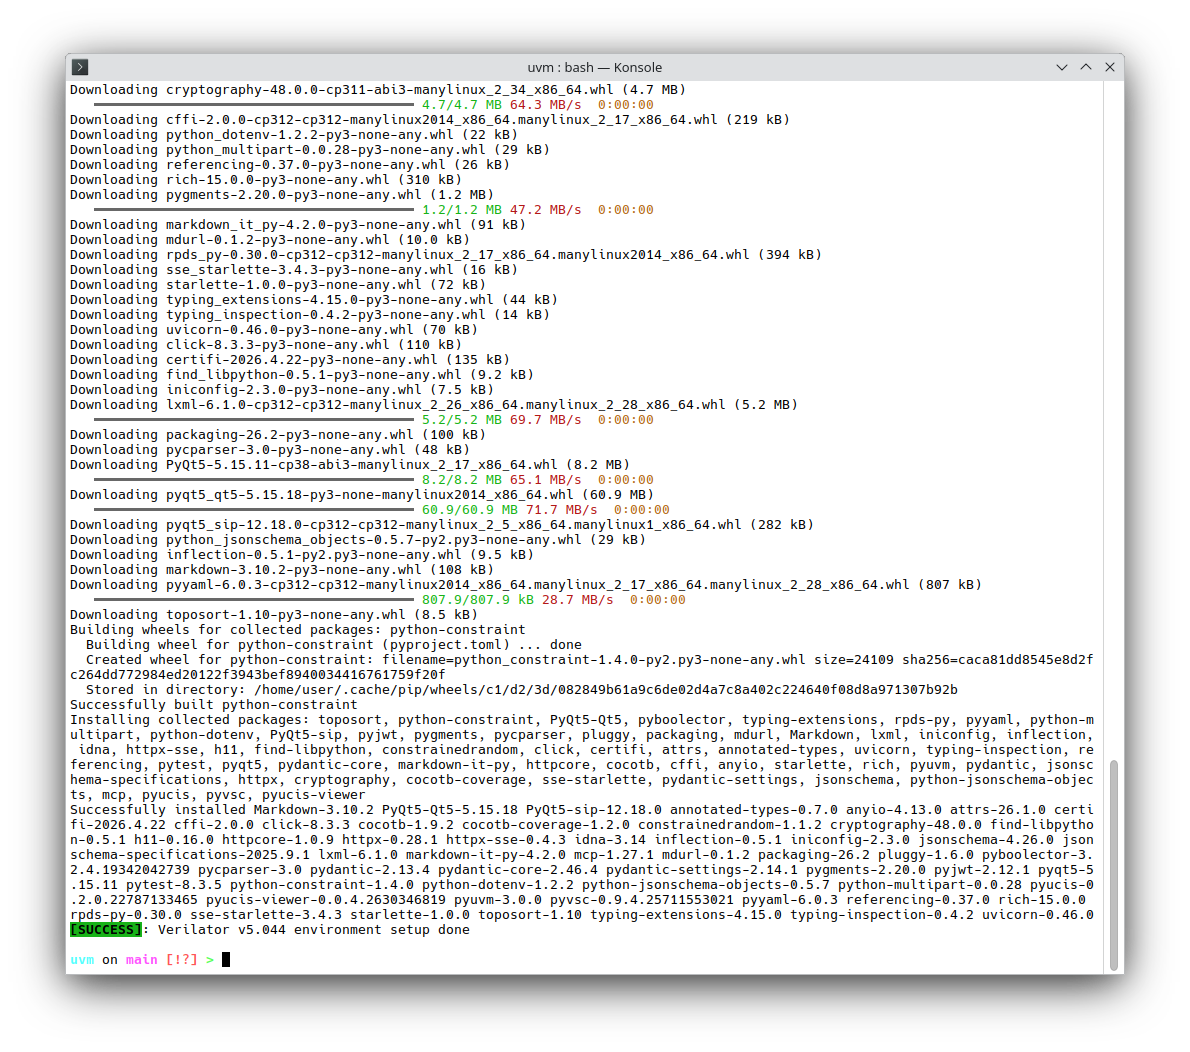
\includegraphics[width=\linewidth]{images/doc_make_venv_verilator.png}
	\caption{Sėkmingas \textit{Verilator} \textit{Python} virtualios aplinkos sąranka naudojant \textit{Make} skriptą}
	\label{fig:doc_make_venv_verilator}
\end{figure}

Po šio žingsnio sistema yra pilnai paruošta testų rašymui ir vykdymui.

\subsection{Naudotojo vadovas}

Šiame skyriuje aprašomi kasdieniai naudotojo veiksmai dirbant su paruošta aplinka. Visas darbas organizuojamas per \textit{GNU Make} komandinę sąsają.

\textbf{Pagalbos iškvietimas} \\
Jei pamiršote komandų sintaksę, bet kuriame \texttt{uvm} katalogo gylyje galite iškviesti pagalbos meniu:
\begin{lstlisting}[basicstyle=\ttfamily\footnotesize, language=bash]
$ make help
\end{lstlisting}

\begin{figure}[H]
	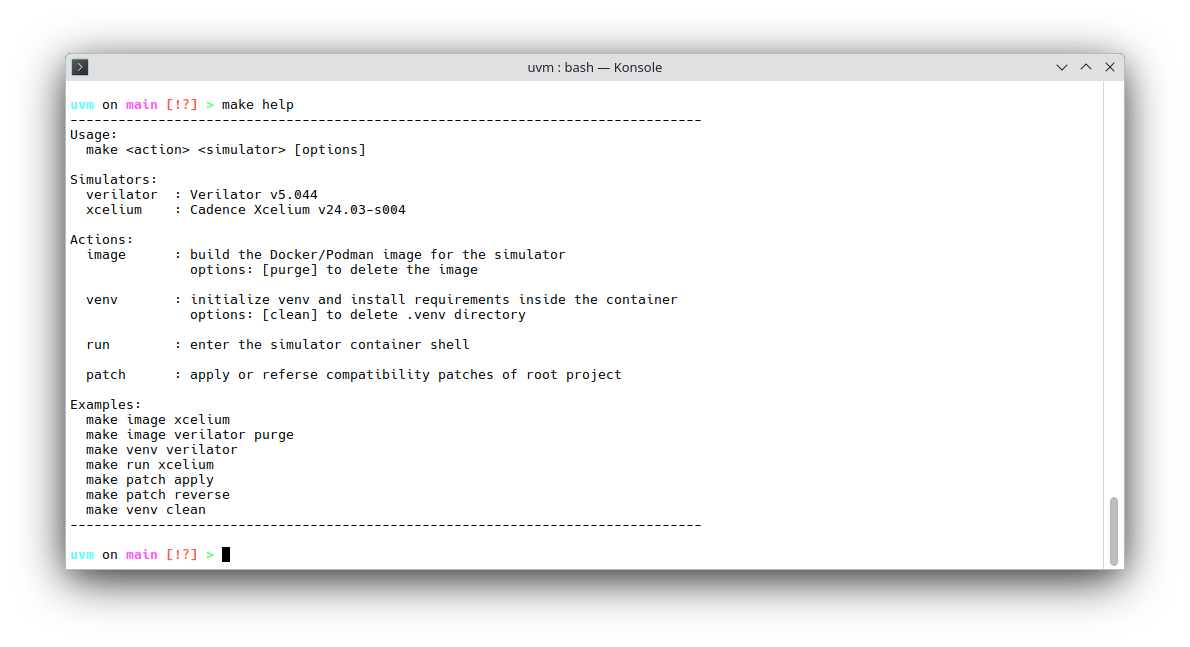
\includegraphics[width=\linewidth]{images/doc_make_help.png}
	\caption{Pagrindinis sistemos pagalbos meniu terminale}
	\label{fig:doc_make_help}
\end{figure}

\textbf{Interaktyvus darbas su Tmux (rekomenduojama)} \\
Kad nereikėtų atidarinėti kelių terminalo langų rankiniu būdu, karkase integruotas \textit{Tmux} sesijų valdiklis. Šis funkcionalumas reikalauja turėti instaliuotą \texttt{tmux v3.0+} įrankį. Paleidus skriptą \texttt{./script/tmux\_env.sh}, jūsų ekranas bus automatiškai padalintas į tris dalis: komandų vykdymo, transakcijų stebėjimo ir imitacijos žurnalo stebėjimo langai. Tarp langų galima naršyti pelės paspaudimu. Sesijos sunaikinimui paspauskite kartu \texttt{Ctrl + B} ir tada kartu \texttt{Shift + X}.

\begin{figure}[H]
	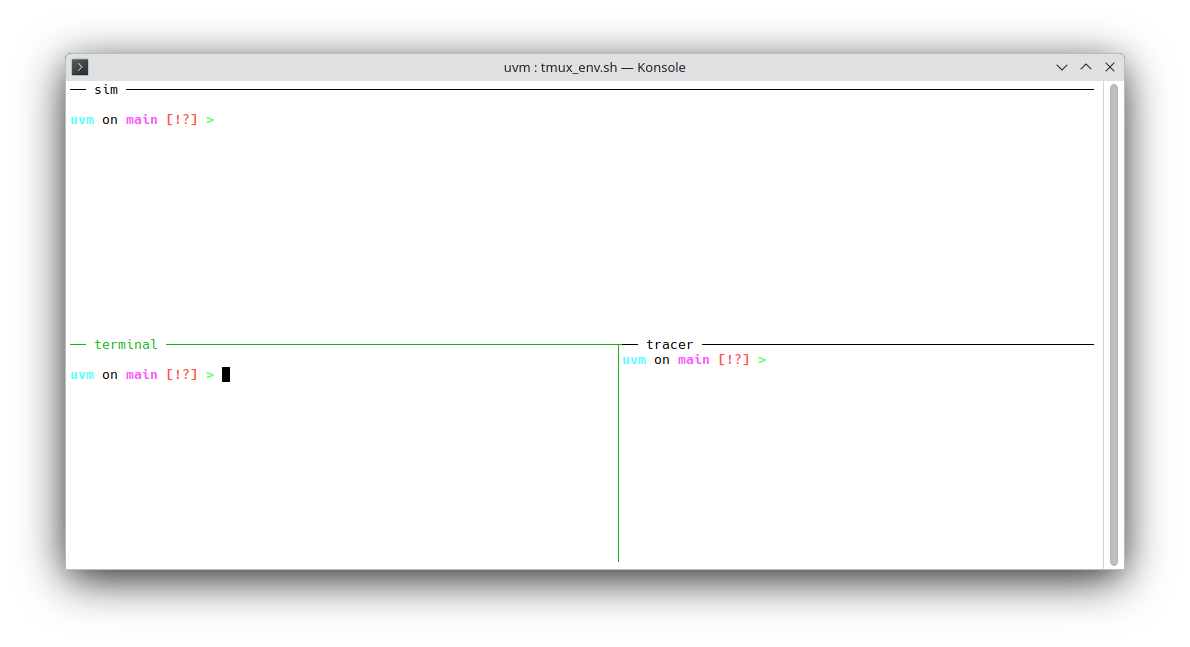
\includegraphics[width=\linewidth]{images/doc_tmux_env.png}
	\caption{Automatizuota \textit{Tmux} kelių polangių darbo aplinka}
	\label{fig:doc_tmux_env}
\end{figure}

\textbf{Testų paleidimas} \\
Testai vykdomi iš \texttt{uvm/sim/} katalogo. Norėdami paleisti konkretų \textit{PyUVM} testą (pavyzdžiui, \texttt{simple\_gpio\_test}) su \textit{Verilator} \glsdisp{simulator}{imituokle}, pirma turite paleisti konteinerį ir tada naudoti testo paleidimo ir konfigūravimo komandą:
\begin{lstlisting}[basicstyle=\ttfamily\footnotesize, language=bash]
$ make run verilator
$ make SIM=verilator TEST=gpio_nibble_mirror_test
\end{lstlisting}

Paleidus, ši komanda automatiškai sukompiliuos \gls{mcu} skirtą C programinę įrangą, atliks \gls{rtl} dizaino sintezę ir paleis virtualius testavimo sekų stimulus. Baigti sekimą reikia terminuoti programą paspaudus \texttt{Ctrl + C}.

\begin{figure}[H]
	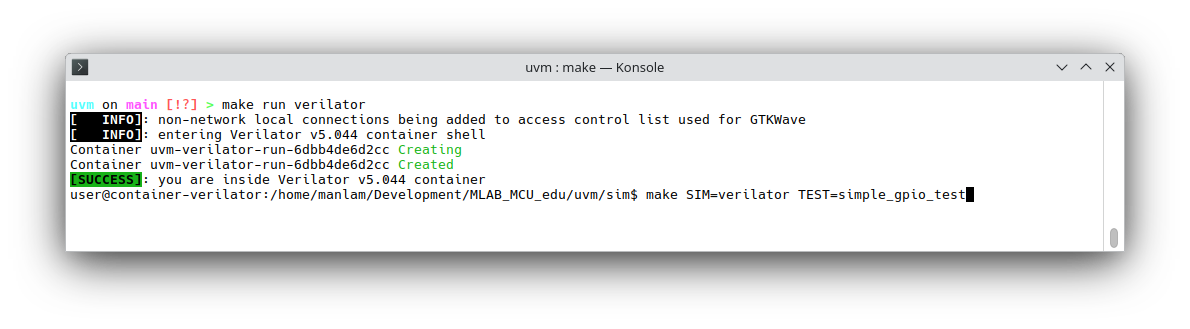
\includegraphics[width=\linewidth]{images/doc_make_run_verilator_test.png}
	\caption{Automatizuota \textit{Tmux} kelių polangių darbo aplinka}
	\label{fig:doc_make_run_verilator_test}
\end{figure}

\textbf{Imitacijos metu vykstančių transakcijų sekimas} \\

Paleidus testą, galima kitame lange atsidaryti transakcijų sekimą:

\begin{lstlisting}[basicstyle=\ttfamily\footnotesize, language=bash]
$ cd sim
$ make tracer
\end{lstlisting}

\begin{figure}[H]
	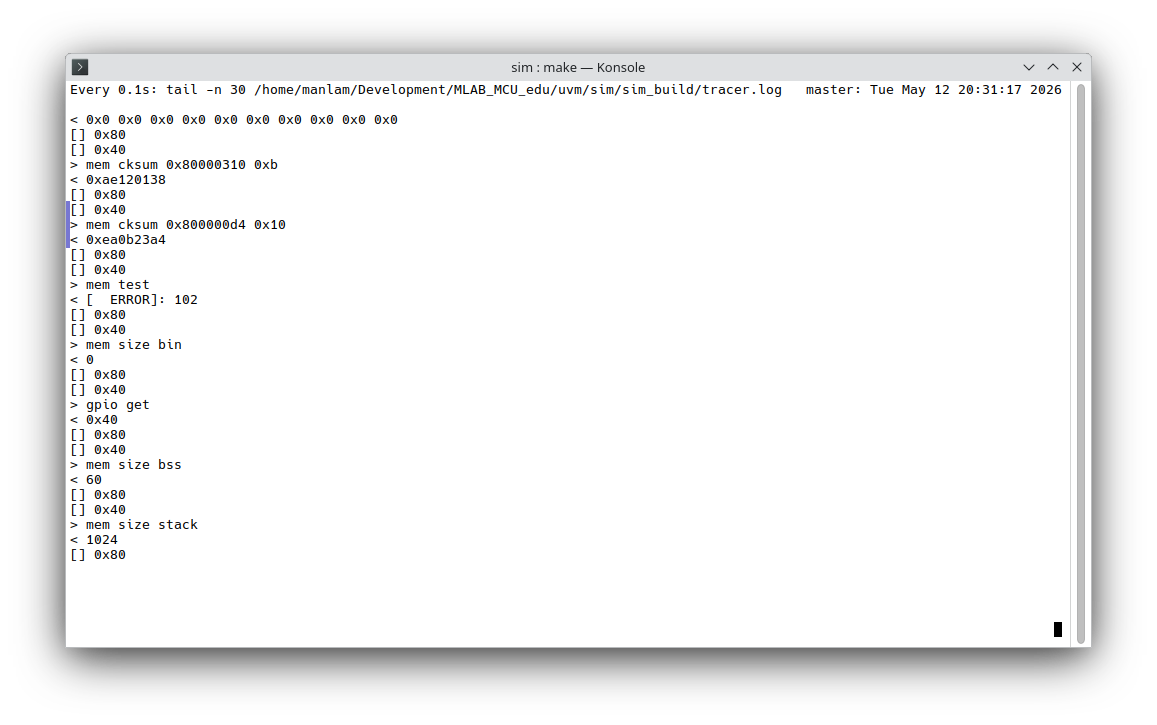
\includegraphics[width=\linewidth]{images/doc_make_tracer.png}
	\caption{Imituojamo testo transakcijų sekimas}
	\label{fig:doc_make_tracer}
\end{figure}

\textbf{Laikinių diagramų peržiūra} \\
Norint vizualiai analizuoti aparatūrinio lygio signalus, testą reikia paleisti su \texttt{WAVES=1} argumentu. Po testo pabaigos, rezultatus atidarykite su komanda \texttt{view}:
\begin{lstlisting}[basicstyle=\ttfamily\footnotesize, language=bash]
$ make SIM=verilator TEST=gpio_nibble_mirror_test WAVES=1
$ cd ..
$ make view verilator waves
\end{lstlisting}
Atsidarys grafinis \textit{GTKWave} (arba \textit{SimVision}) langas. \textit{Pastaba: tam reikalinga X11 langų serverio integracija jūsų kompiuteryje (pvz., Xming Windows sistemoje, jei naudojate WSL).}

\begin{figure}[H]
	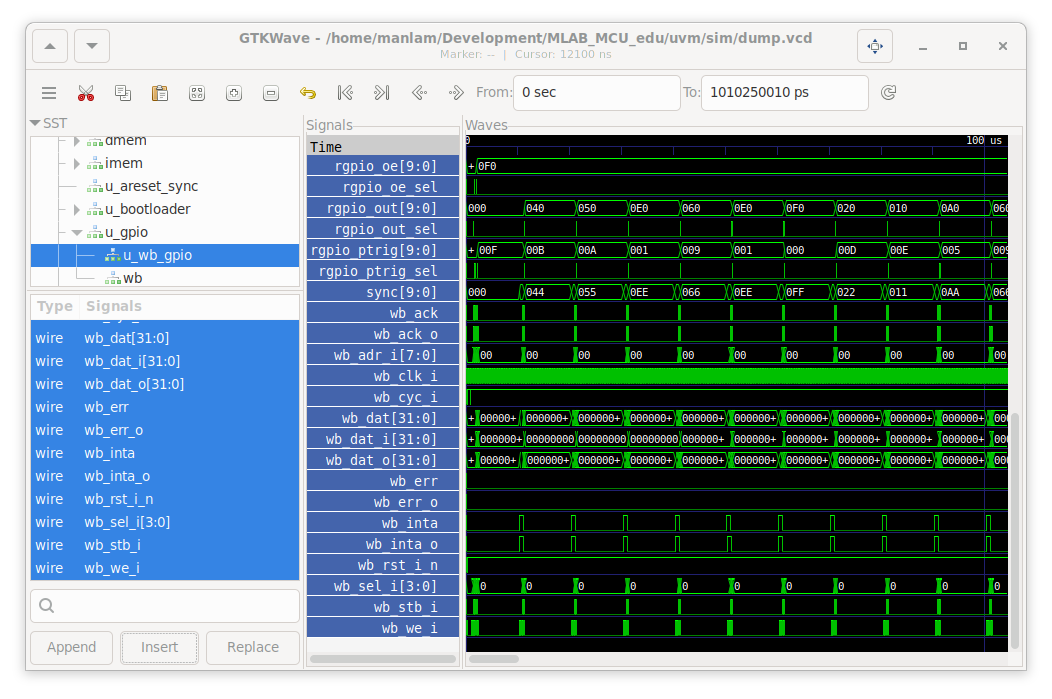
\includegraphics[width=\linewidth]{images/doc_make_view_verilator_waves.png}
	\caption{Signalų laikinės diagramos peržiūra \textit{GTKWave} įrankyje}
	\label{fig:doc_make_view_verilator_waves}
\end{figure}

\textbf{Galimų klaidų sprendimai:}
\begin{itemize}
	\item \textit{Klaida: „docker requires sudo, is not running...“} -- Įsitikinkite, kad jūsų naudotojas priklauso \texttt{docker} grupei (\texttt{sudo usermod -aG docker \$USER}) arba kad \textit{Docker} tarnyba yra aktyvi.
	\item \textit{Klaida: „python's virtual environment not activated“} -- Prieš leidžiant komandas \texttt{sim} kataloge, terminale įvykdykite \texttt{source ../.venv/bin/activate}.
\end{itemize}


\subsection{Administravimo vadovas}

Šis poskyris skirtas organizacijos IT administratoriams, kurie atsakingi už komercinės testavimo infrastruktūros parengimą. Skirtingai nei atviros prieigos \textit{Verilator} aplinka, \textit{Cadence Xcelium} įrankių palaikymas reikalauja specifinės serverinės aplinkos konfigūracijos.

\textbf{Serverio reikalavimai:}
\begin{itemize}
	\item \textbf{Aparatinė įranga:} Serverinis x86\_64 architektūros procesorius, mažiausiai 32 GB RAM ir bent 10 GB laisvos vietos diske.
	\item \textbf{Operacinė sistema:} \textit{Rocky Linux 8.1} (arba atitikmuo -- \textit{RHEL 8.1}). Tai būtina, nes \textit{Cadence} teikia pilną palaikymą ir stabilumo garantijas tik šioje \textit{Linux} distribucijų šeimoje.
	\item \textbf{Konteinerių variklis:} \textit{Podman} (rekomenduojama vietoje \textit{Docker} dėl geresnės \textit{rootless} integracijos \textit{RHEL} sistemose), kuris įdiegiamas kartu su \textit{Rocky Linux 8.1} operacine sistema.
\end{itemize}

\textbf{EDA įrankių ir licencijų konfigūravimas:} \\
Karkasas \textit{Cadence Xcelium} ir \textit{SimVision} įrankių pats neįdiegia -- juos turi instaliuoti administratorius pagal oficialią gamintojo dokumentaciją į pasirinktą serverio katalogą, karkaso naudojamas katalogas yra \texttt{/eda/cadence/2024-25/}. 

Siekiant užtikrinti, kad konteinerizuoti \textit{Python} \gls{uvm} skriptai galėtų pasiekti licencijuotą įrangą, administratorius naudotojų aplinkos (\texttt{.bashrc} ar \texttt{.bash\_profile}) lygmenyje privalo eksportuoti šiuos aplinkos kintamuosius:
\begin{lstlisting}[basicstyle=\ttfamily\footnotesize, language=bash]
# Export full path to xcelium binaries
export CADENCE_PATH=/eda/cadence/2024-25/RHELx86/XCELIUM_24.03.004

# Export license file
export CDS_LIC_FILE=5280@server_licence_or_ip_address
\end{lstlisting}
Konteinerio atvaizdo surinkimo (\texttt{make image xcelium}) ir paleidimo (\texttt{make run xcelium}) metu, pagrindinis karkaso \textit{Makefile} skriptas šiuos kintamuosius dinamiškai perduoda į izoliuotą \textit{Podman} aplinką. Tai leidžia \textit{Cocotb} karkasui dinamiškai užkrauti \textit{Xcelium} vykdomuosius failus tiesiai iš serverio (angl. \textit{read-only mount} principu), nepažeidžiant gamintojo licencijavimo sąlygų.